% TEX PROGRAM = xelatex
\documentclass[UTF8]{ctexart}
    \title{求最小生成树}
    \author{2017211123 褚逸豪}
    \usepackage{tikz}
    \usepackage{amsmath}
    \usepackage{amssymb}
    \usepackage{multicol}
    \usepackage{geometry}
    \geometry{a4paper,scale=0.7}
    \usetikzlibrary{arrows,patterns}
	\tikzset{mn/.append style={minimum size=0.5cm, draw,circle,inner sep=0.05cm}}
    \tikzset{gg/.append style={pattern=dots}}
    \pgfdeclarepatternformonly{soft crosshatch}{\pgfqpoint{-1pt}{-1pt}}{\pgfqpoint{4pt}{4pt}}{\pgfqpoint{3pt}{3pt}}%
    {
        \pgfsetstrokeopacity{0.3}
        \pgfsetlinewidth{0.4pt}
        \pgfpathmoveto{\pgfqpoint{3.1pt}{0pt}}
        \pgfpathlineto{\pgfqpoint{0pt}{3.1pt}}
        \pgfpathmoveto{\pgfqpoint{0pt}{0pt}}
        \pgfpathlineto{\pgfqpoint{3.1pt}{3.1pt}}
        \pgfusepath{stroke}
    }
\begin{document}
    \maketitle
    \section{初始图}
    \begin{center}
        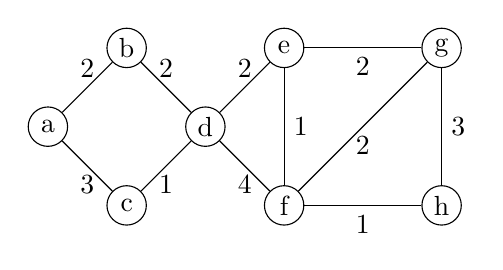
\begin{tikzpicture}
            % \SetUpVertex
            \node[mn] (a) at (0,0) {a};
            \node[mn] (b) at (1,1) {b};
            \node[mn] (c) at (1,-1) {c};
            \node[mn] (d) at (2,0) {d};
            \node[mn] (e) at (3,1) {e};
            \node[mn] (f) at (3,-1) {f};
            \node[mn] (g) at (5,1) {g};
            \node[mn] (h) at (5,-1) {h};
            \path (a) edge node[above]{2} (b) edge node[below]{3} (c);
            \path (d) edge node[above]{2} (b) edge node[below]{1} (c);
            \path (e) edge node[above]{2} (d) edge node[auto]{1} (f);
            \path (f) edge node[below]{4} (d) edge node[below]{1} (h);
            \path (g) edge node[below]{2} (f) edge node[auto]{3} (h) edge node[below]{2} (e);
            % \edge node[auto](a1) node
        \end{tikzpicture}
    \end{center}
    \section{Prim求最小生成树}
    \begin{center}
        \noindent 先取$a$为起始点
        \begin{center}
            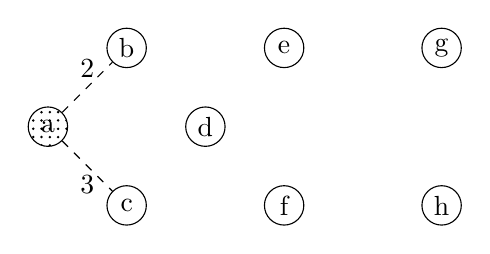
\begin{tikzpicture}
                % \SetUpVertex
                \node[mn,gg] (a) at (0,0) {a};
                \node[mn] (b) at (1,1) {b};
                \node[mn] (c) at (1,-1) {c};
                \node[mn] (d) at (2,0) {d};
                \node[mn] (e) at (3,1) {e};
                \node[mn] (f) at (3,-1) {f};
                \node[mn] (g) at (5,1) {g};
                \node[mn] (h) at (5,-1) {h};
                \path (a) edge[dashed] node[above]{2} (b) edge[dashed] node[below]{3} (c);
            \end{tikzpicture}
        \end{center}
        接着扩展$b$
        \begin{center}
            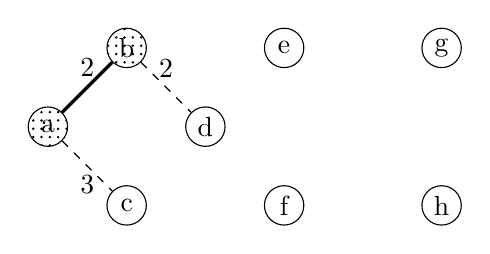
\begin{tikzpicture}
                % \SetUpVertex
                \node[mn,gg] (a) at (0,0) {a};
                \node[mn,gg] (b) at (1,1) {b};
                \node[mn] (c) at (1,-1) {c};
                \node[mn] (d) at (2,0) {d};
                \node[mn] (e) at (3,1) {e};
                \node[mn] (f) at (3,-1) {f};
                \node[mn] (g) at (5,1) {g};
                \node[mn] (h) at (5,-1) {h};
                \path (a) edge[very thick] node[above]{2} (b) edge[dashed] node[below]{3} (c);
                \path (b) edge[dashed] node[above]{2} (d);
            \end{tikzpicture}
        \end{center}
        然后扩展$d$
        \begin{center}
            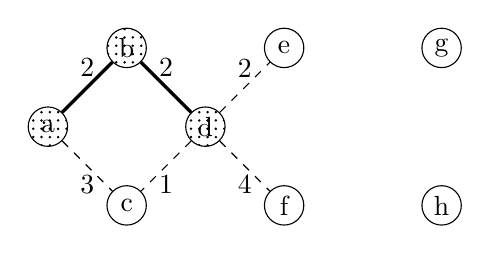
\begin{tikzpicture}
                % \SetUpVertex
                \node[mn,gg] (a) at (0,0) {a};
                \node[mn,gg] (b) at (1,1) {b};
                \node[mn] (c) at (1,-1) {c};
                \node[mn,gg] (d) at (2,0) {d};
                \node[mn] (e) at (3,1) {e};
                \node[mn] (f) at (3,-1) {f};
                \node[mn] (g) at (5,1) {g};
                \node[mn] (h) at (5,-1) {h};
                \path (a) edge[very thick] node[above]{2} (b) edge[dashed] node[below]{3} (c);
                \path (b) edge[very thick] node[above]{2} (d);
                \path (d) edge[dashed] node[below]{1} (c) edge[dashed] node[above]{2} (e) edge[dashed] node[below]{4} (f);
            \end{tikzpicture}
        \end{center}
        扩展$c$,紧接着扩展$e$
        \begin{center}
            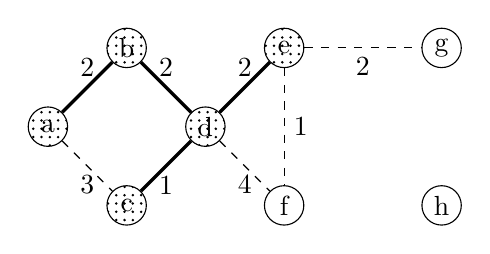
\begin{tikzpicture}
                % \SetUpVertex
                \node[mn,gg] (a) at (0,0) {a};
                \node[mn,gg] (b) at (1,1) {b};
                \node[mn,gg] (c) at (1,-1) {c};
                \node[mn,gg] (d) at (2,0) {d};
                \node[mn,gg] (e) at (3,1) {e};
                \node[mn] (f) at (3,-1) {f};
                \node[mn] (g) at (5,1) {g};
                \node[mn] (h) at (5,-1) {h};
                \path (a) edge[very thick] node[above]{2} (b) edge[dashed] node[below]{3} (c);
                \path (b) edge[very thick] node[above]{2} (d);
                \path (d) edge[very thick] node[below]{1} (c) edge[very thick] node[above]{2} (e) edge[dashed] node[below]{4} (f);
                \path (e) edge[dashed] node[below]{2} (g) edge[dashed] node[auto]{1} (f);
            \end{tikzpicture}
        \end{center}
        然后我们扩展$f$
        \begin{center}
            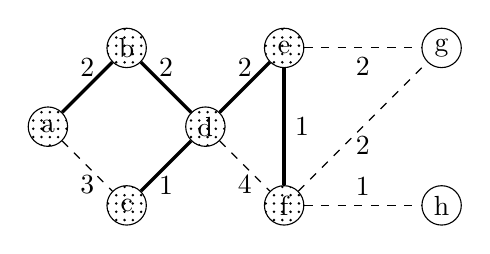
\begin{tikzpicture}
                % \SetUpVertex
                \node[mn,gg] (a) at (0,0) {a};
                \node[mn,gg] (b) at (1,1) {b};
                \node[mn,gg] (c) at (1,-1) {c};
                \node[mn,gg] (d) at (2,0) {d};
                \node[mn,gg] (e) at (3,1) {e};
                \node[mn,gg] (f) at (3,-1) {f};
                \node[mn] (g) at (5,1) {g};
                \node[mn] (h) at (5,-1) {h};
                \path (a) edge[very thick] node[above]{2} (b) edge[dashed] node[below]{3} (c);
                \path (b) edge[very thick] node[above]{2} (d);
                \path (d) edge[very thick] node[below]{1} (c) edge[very thick] node[above]{2} (e) edge[dashed] node[below]{4} (f);
                \path (e) edge[dashed] node[below]{2} (g) edge[very thick] node[auto]{1} (f);
                \path (f) edge[dashed] node[above]{1} (h) edge[dashed] node[below]{2} (g);
            \end{tikzpicture}
        \end{center}
        扩展$h$
        \begin{center}
            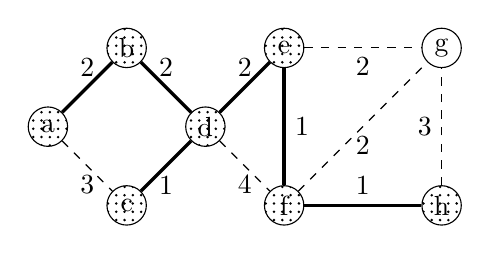
\begin{tikzpicture}
                % \SetUpVertex
                \node[mn,gg] (a) at (0,0) {a};
                \node[mn,gg] (b) at (1,1) {b};
                \node[mn,gg] (c) at (1,-1) {c};
                \node[mn,gg] (d) at (2,0) {d};
                \node[mn,gg] (e) at (3,1) {e};
                \node[mn,gg] (f) at (3,-1) {f};
                \node[mn] (g) at (5,1) {g};
                \node[mn,gg] (h) at (5,-1) {h};
                \path (a) edge[very thick] node[above]{2} (b) edge[dashed] node[below]{3} (c);
                \path (b) edge[very thick] node[above]{2} (d);
                \path (d) edge[very thick] node[below]{1} (c) edge[very thick] node[above]{2} (e) edge[dashed] node[below]{4} (f);
                \path (e) edge[dashed] node[below]{2} (g) edge[very thick] node[auto]{1} (f);
                \path (f) edge[very thick] node[above]{1} (h) edge[dashed] node[below]{2} (g);
                \path (h) edge[dashed] node[auto]{3} (g);
            \end{tikzpicture}
        \end{center}
        最后吸纳$g$
        \begin{center}
            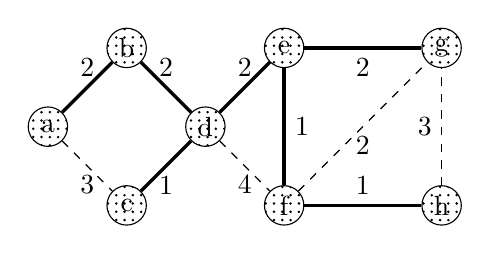
\begin{tikzpicture}
                % \SetUpVertex
                \node[mn,gg] (a) at (0,0) {a};
                \node[mn,gg] (b) at (1,1) {b};
                \node[mn,gg] (c) at (1,-1) {c};
                \node[mn,gg] (d) at (2,0) {d};
                \node[mn,gg] (e) at (3,1) {e};
                \node[mn,gg] (f) at (3,-1) {f};
                \node[mn,gg] (g) at (5,1) {g};
                \node[mn,gg] (h) at (5,-1) {h};
                \path (a) edge[very thick] node[above]{2} (b) edge[dashed] node[below]{3} (c);
                \path (b) edge[very thick] node[above]{2} (d);
                \path (d) edge[very thick] node[below]{1} (c) edge[very thick] node[above]{2} (e) edge[dashed] node[below]{4} (f);
                \path (e) edge[very thick] node[below]{2} (g) edge[very thick] node[auto]{1} (f);
                \path (f) edge[very thick] node[above]{1} (h) edge[dashed] node[below]{2} (g);
                \path (h) edge[dashed] node[auto]{3} (g);
            \end{tikzpicture}
        \end{center}
        我们得到了如下的最小生成树
        \begin{center}
            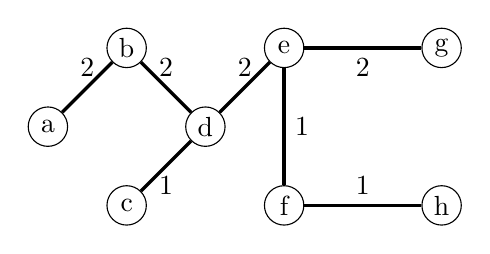
\begin{tikzpicture}
                % \SetUpVertex
                \node[mn] (a) at (0,0) {a};
                \node[mn] (b) at (1,1) {b};
                \node[mn] (c) at (1,-1) {c};
                \node[mn] (d) at (2,0) {d};
                \node[mn] (e) at (3,1) {e};
                \node[mn] (f) at (3,-1) {f};
                \node[mn] (g) at (5,1) {g};
                \node[mn] (h) at (5,-1) {h};
                \path (a) edge[very thick] node[above]{2} (b) ;
                \path (b) edge[very thick] node[above]{2} (d);
                \path (d) edge[very thick] node[below]{1} (c) edge[very thick] node[above]{2} (e);
                \path (e) edge[very thick] node[below]{2} (g) edge[very thick] node[auto]{1} (f);
                \path (f) edge[very thick] node[above]{1} (h);
            \end{tikzpicture}
        \end{center}
    \end{center}
    \section{Kruskal求最小生成树}
    \noindent 先将图中的边按权值递增序排序
    \begin{multicols}{2}
        \begin{enumerate}
            \item c-d:1
            \item e-f:1
            \item f-h:1
            \item b-d:2
            \item d-e:2
            \item e-g:2
            \item g-f:2
            \item a-b:2
            \item a-c:3
            \item g-h:3
            \item d-f:4
        \end{enumerate}
    \end{multicols}
    \begin{center}
        \noindent 尝试并加入第一条边
        \begin{center}
            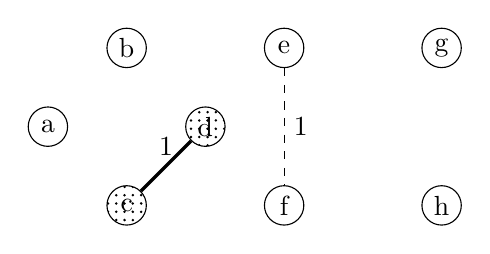
\begin{tikzpicture}
                % \SetUpVertex
                \node[mn] (a) at (0,0) {a};
                \node[mn] (b) at (1,1) {b};
                \node[mn,gg] (c) at (1,-1) {c};
                \node[mn,gg] (d) at (2,0) {d};
                \node[mn] (e) at (3,1) {e};
                \node[mn] (f) at (3,-1) {f};
                \node[mn] (g) at (5,1) {g};
                \node[mn] (h) at (5,-1) {h};
                \path (c) edge[very thick] node[above]{1} (d);
                \path (e) edge[dashed] node[auto]{1} (f);
            \end{tikzpicture}
        \end{center}
        加入第二条,准备插入第三条
        \begin{center}
            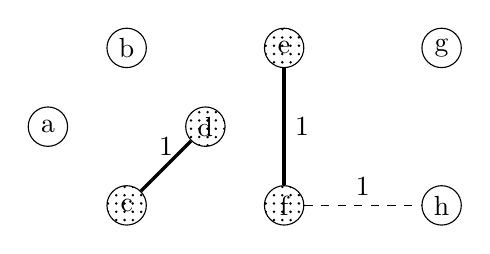
\begin{tikzpicture}
                % \SetUpVertex
                \node[mn] (a) at (0,0) {a};
                \node[mn] (b) at (1,1) {b};
                \node[mn,gg] (c) at (1,-1) {c};
                \node[mn,gg] (d) at (2,0) {d};
                \node[mn,gg] (e) at (3,1) {e};
                \node[mn,gg] (f) at (3,-1) {f};
                \node[mn] (g) at (5,1) {g};
                \node[mn] (h) at (5,-1) {h};
                \path (c) edge[very thick] node[above]{1} (d);
                \path (e) edge[very thick] node[auto]{1} (f);
                \path (f) edge[dashed] node[auto]{1} (h);
            \end{tikzpicture}
        \end{center}
        插入第三条,尝试第四条
        \begin{center}
            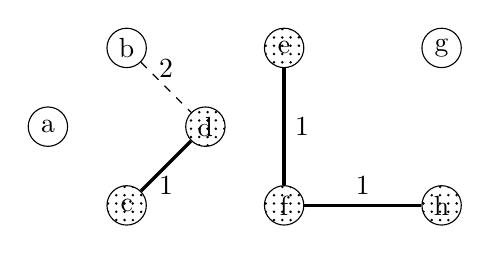
\begin{tikzpicture}
                % \SetUpVertex
                \node[mn] (a) at (0,0) {a};
                \node[mn] (b) at (1,1) {b};
                \node[mn,gg] (c) at (1,-1) {c};
                \node[mn,gg] (d) at (2,0) {d};
                \node[mn,gg] (e) at (3,1) {e};
                \node[mn,gg] (f) at (3,-1) {f};
                \node[mn] (g) at (5,1) {g};
                \node[mn,gg] (h) at (5,-1) {h};
                \path (c) edge[very thick] node[below]{1} (d);
                \path (e) edge[very thick] node[auto]{1} (f);
                \path (f) edge[very thick] node[auto]{1} (h);
                \path (b) edge[dashed] node[above]{2} (d);
            \end{tikzpicture}
        \end{center}
        插入第四条,尝试第五条
        \begin{center}
            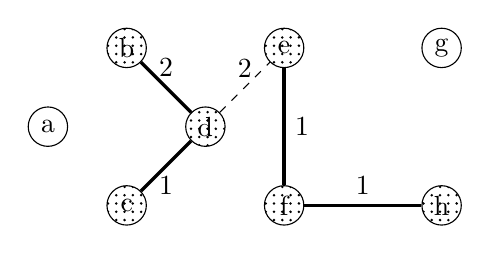
\begin{tikzpicture}
                % \SetUpVertex
                \node[mn] (a) at (0,0) {a};
                \node[mn,gg] (b) at (1,1) {b};
                \node[mn,gg] (c) at (1,-1) {c};
                \node[mn,gg] (d) at (2,0) {d};
                \node[mn,gg] (e) at (3,1) {e};
                \node[mn,gg] (f) at (3,-1) {f};
                \node[mn] (g) at (5,1) {g};
                \node[mn,gg] (h) at (5,-1) {h};
                \path (c) edge[very thick] node[below]{1} (d);
                \path (e) edge[very thick] node[auto]{1} (f);
                \path (f) edge[very thick] node[auto]{1} (h);
                \path (b) edge[very thick] node[above]{2} (d);
                \path (d) edge[dashed] node[above]{2} (e);
            \end{tikzpicture}
        \end{center}
        插入第五条,尝试第六条
        \begin{center}
            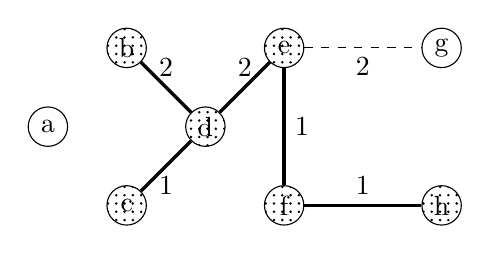
\begin{tikzpicture}
                % \SetUpVertex
                \node[mn] (a) at (0,0) {a};
                \node[mn,gg] (b) at (1,1) {b};
                \node[mn,gg] (c) at (1,-1) {c};
                \node[mn,gg] (d) at (2,0) {d};
                \node[mn,gg] (e) at (3,1) {e};
                \node[mn,gg] (f) at (3,-1) {f};
                \node[mn] (g) at (5,1) {g};
                \node[mn,gg] (h) at (5,-1) {h};
                \path (c) edge[very thick] node[below]{1} (d);
                \path (e) edge[very thick] node[auto]{1} (f);
                \path (f) edge[very thick] node[auto]{1} (h);
                \path (b) edge[very thick] node[above]{2} (d);
                \path (d) edge[very thick] node[above]{2} (e);
                \path (e) edge[dashed] node[below]{2} (g);
            \end{tikzpicture}
        \end{center}
        插入第六条,在尝试第七条边的时候发现第七条边不合法
        \begin{center}
            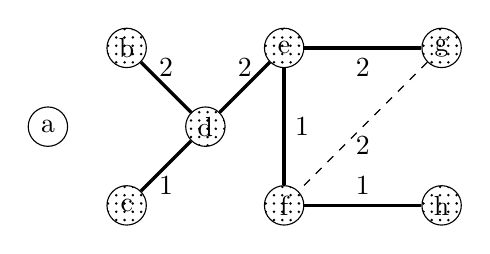
\begin{tikzpicture}
                % \SetUpVertex
                \node[mn] (a) at (0,0) {a};
                \node[mn,gg] (b) at (1,1) {b};
                \node[mn,gg] (c) at (1,-1) {c};
                \node[mn,gg] (d) at (2,0) {d};
                \node[mn,gg] (e) at (3,1) {e};
                \node[mn,gg] (f) at (3,-1) {f};
                \node[mn,gg] (g) at (5,1) {g};
                \node[mn,gg] (h) at (5,-1) {h};
                \path (c) edge[very thick] node[below]{1} (d);
                \path (e) edge[very thick] node[auto]{1} (f);
                \path (f) edge[very thick] node[auto]{1} (h);
                \path (b) edge[very thick] node[above]{2} (d);
                \path (d) edge[very thick] node[above]{2} (e);
                \path (e) edge[very thick] node[below]{2} (g);
                \path (g) edge[dashed] node[below]{2} (f);
            \end{tikzpicture}
        \end{center}
        尝试第八条,合法,加入之
        \begin{center}
            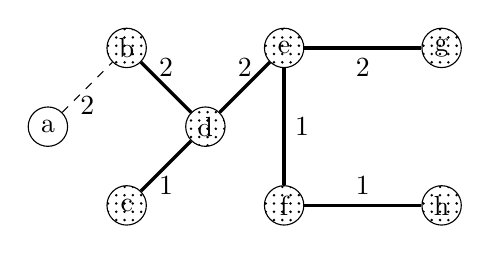
\begin{tikzpicture}
                % \SetUpVertex
                \node[mn] (a) at (0,0) {a};
                \node[mn,gg] (b) at (1,1) {b};
                \node[mn,gg] (c) at (1,-1) {c};
                \node[mn,gg] (d) at (2,0) {d};
                \node[mn,gg] (e) at (3,1) {e};
                \node[mn,gg] (f) at (3,-1) {f};
                \node[mn,gg] (g) at (5,1) {g};
                \node[mn,gg] (h) at (5,-1) {h};
                \path (c) edge[very thick] node[below]{1} (d);
                \path (e) edge[very thick] node[auto]{1} (f);
                \path (f) edge[very thick] node[auto]{1} (h);
                \path (b) edge[very thick] node[above]{2} (d);
                \path (d) edge[very thick] node[above]{2} (e);
                \path (e) edge[very thick] node[below]{2} (g);
                \path (a) edge[dashed] node[below]{2} (b);
            \end{tikzpicture}
        \end{center}
        最后我们得到了如下最小生成树
        \begin{center}
            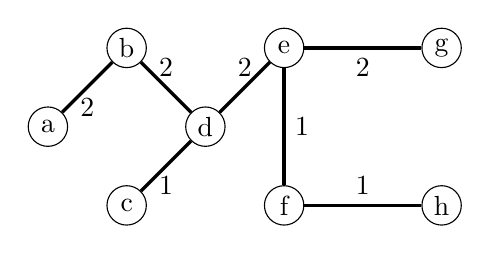
\begin{tikzpicture}
                % \SetUpVertex
                \node[mn] (a) at (0,0) {a};
                \node[mn] (b) at (1,1) {b};
                \node[mn] (c) at (1,-1) {c};
                \node[mn] (d) at (2,0) {d};
                \node[mn] (e) at (3,1) {e};
                \node[mn] (f) at (3,-1) {f};
                \node[mn] (g) at (5,1) {g};
                \node[mn] (h) at (5,-1) {h};
                \path (c) edge[very thick] node[below]{1} (d);
                \path (e) edge[very thick] node[auto]{1} (f);
                \path (f) edge[very thick] node[auto]{1} (h);
                \path (b) edge[very thick] node[above]{2} (d);
                \path (d) edge[very thick] node[above]{2} (e);
                \path (e) edge[very thick] node[below]{2} (g);
                \path (a) edge[very thick] node[below]{2} (b);
            \end{tikzpicture}
        \end{center}
    \end{center}
\end{document}